\documentclass[12pt, a4paper]{article}

\usepackage{mathpazo}
\usepackage[T1]{fontenc}

\usepackage{microtype}
\usepackage{geometry}
\geometry{top=1.1in, bottom=1.1in, left=1.25in, right=1.25in}

\usepackage{setspace}
\onehalfspacing

\usepackage{amsmath, amssymb}
\usepackage{physics}
\usepackage{graphicx}
\usepackage{tikz}
\usetikzlibrary{arrows.meta, positioning, calc}
\usepackage{hyperref}

\hypersetup{
  colorlinks=true,
  linkcolor=black,
  citecolor=black,
  urlcolor=black
}

\title{\large\textbf{The Caldera Reactor:\\
Thermopneumatic Compression, Fluidic Computation,\\
and Adaptive Biomass Processing}}

\author{Flyxion\\
\small Independent Researcher}

\date{\today}

\begin{document}

\maketitle

\begin{abstract}
The Caldera Reactor is a thermopneumatic compression system for cyclic processing of wet biomass into biocrude and biochemical derivatives. The system integrates tidal and geothermal energy inputs with a vertically actuated press cycle, adaptive fluid routing, and biologically mediated catalysis. Central to its operation is a thermofluidic computation layer, implemented via a pressure-sensitive knot lattice that performs decentralized control. This paper formalizes the reactor dynamics, extends its computational interpretation through a variational field-theoretic formulation, and establishes a structural equivalence with the Relativistic Scalar--Vector Plenum (RSVP) framework, proposing a unified account of its physical and informational behavior.
\end{abstract}

\section{Introduction}

The processing of wet biomass presents a persistent engineering challenge due to high water content, heterogeneous composition, and energy-intensive conversion pathways. The Caldera Reactor addresses these constraints by combining thermodynamic cycling, mechanical compression, and adaptive control into a closed-loop system. Unlike conventional reactors, the Caldera system embeds computation directly into its fluidic structure, allowing real-time adaptation without centralized control and making it both energetically efficient and structurally scalable.

This paper proceeds through three levels of formalization. We first reconstruct the system's engineering dynamics, specifying the governing equations for each operational phase. We then extend the thermofluidic computation layer into a variational field-theoretic object, showing that the discrete switching behavior of the knot lattice emerges from gradient descent in a continuous energy functional. Finally, we establish a structural equivalence between the reactor dynamics and the RSVP framework, reinterpreting the system as a physical instantiation of coupled scalar--vector--constraint field dynamics. Each level of description is intended to deepen rather than replace the others.

\section{System Architecture}

The reactor consists of a vertically actuated compression plate, sub-Caldera lift channels, and a network of energy recovery turbines. Biomass inputs are layered mixtures of kelp, peat, and sediment. The system operates as a cyclic process in which a lift phase, a clamp-and-draw phase, a press phase, and a recovery phase succeed one another continuously:
\[
\text{Lift} \;\rightarrow\; \text{Clamp/Draw} \;\rightarrow\; \text{Press} \;\rightarrow\; \text{Recovery}
\]
\begin{figure}[h]
\centering
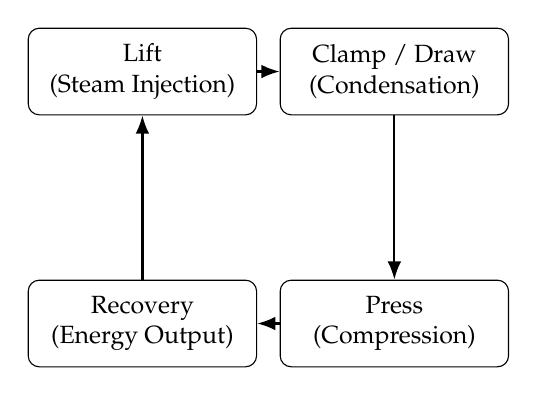
\begin{tikzpicture}[
    node distance=3.2cm,
    every node/.style={draw, rectangle, rounded corners, minimum width=2.9cm, minimum height=1.1cm, align=center, font=\small},
    arrow/.style={-{Latex}, thick}
]
\node (lift) {Lift\\(Steam Injection)};
\node (draw) [right of=lift] {Clamp / Draw\\(Condensation)};
\node (press) [below of=draw] {Press\\(Compression)};
\node (recover) [left of=press] {Recovery\\(Energy Output)};
\draw[arrow] (lift) -- (draw);
\draw[arrow] (draw) -- (press);
\draw[arrow] (press) -- (recover);
\draw[arrow] (recover) -- (lift);
\end{tikzpicture}
\caption{Cyclic operation of the Caldera Reactor. Each phase corresponds to a coordinated transformation in pressure, volume, and material state; transitions are governed by the internal dynamics of the fluidic network.}
\end{figure}

Each phase corresponds to a coordinated transformation in pressure, volume, and material state, with the transitions between phases governed not by external command but by the internal dynamics of the fluidic network.

\section{Lift Phase Dynamics}

Superheated steam is injected beneath the Caldera plate, generating an upward force according to:
\[
F_{\text{lift}} = A_p \bigl(P_{\text{steam}} - P_{\text{upper}}\bigr) - F_{\text{resistive}}
\]
The pressure evolution in the sub-plate volume follows:
\[
\frac{dP}{dt} = \frac{RT}{V} \left( \frac{dm}{dt} \right) - \frac{\gamma P}{V} \frac{dV}{dt}
\]
This equation couples thermodynamic expansion with mass injection, producing a controlled vertical displacement. The resistive term $F_{\text{resistive}}$ encodes the combined inertial, frictional, and hydrostatic loads on the plate.

\section{Clamp and Draw Phase}

Cooling induces condensation, generating a pressure differential that draws the plate downward and introduces seawater inflow:
\[
F_{\text{vacuum}} = A_{\text{inlet}} \bigl(P_{\text{external}} - P_{\text{collapsed}}\bigr)
\]
This phase simultaneously seals the compression chamber and redistributes internal mass in preparation for the press. Fluid routing during this phase is governed by a pressure-sensitive knot lattice, which operates as a distributed switching system embedded in the physical structure of the reactor.

\subsection{Knot Lattice Switching}

The fluidic network is governed by discrete pressure thresholds at each lattice node $x$:
\[
K(x,t) =
\begin{cases}
\phantom{-}1 & \text{if } P_x(t) > P_{\text{high}} \\
-1 & \text{if } P_x(t) < P_{\text{low}} \\
\phantom{-}0 & \text{otherwise}
\end{cases}
\]
This creates a ternary logic system embedded directly in the physical substrate. The three states correspond respectively to active forward routing, active reverse routing, and a passive or transitional configuration. Because the switching condition is determined entirely by local pressure values, no external controller needs to interrogate or command individual nodes; the network collectively resolves a routing configuration from local pressure information alone.

\section{Press Phase and Material Response}

Compression induces viscoelastic deformation in the layered biomass:
\[
\sigma(t) = E_{\text{eff}}\, \epsilon(t) + \eta\, \frac{d\epsilon}{dt}
\]
The effective modulus $E_{\text{eff}}$ and viscosity $\eta$ depend on the current composition and hydration state of the biomass column. This constitutive relation governs the rate of biocrude extraction and the progressive restructuring of material phases across the press cycle. As compression proceeds, the material transitions from a porous, highly hydrated medium to a denser, partially dewatered residue, with the expelled liquid carrying dissolved biochemical fractions into the recovery channels.

\section{Energy Recovery}

Energy is recovered via gravitational descent of the plate and turbine coupling in the outflow channels:
\[
E_{\text{rec}} = \int_{h_0}^{h_f} \eta_{\text{turbine}}\, \rho_w\, g\, A\, h\; dh
\]
This partial recycling of mechanical work reduces the net energy cost of the press cycle. The efficiency factor $\eta_{\text{turbine}}$ captures parasitic losses in the turbine coupling; the integral over plate descent height $h$ from initial position $h_0$ to final position $h_f$ gives the total recoverable energy per cycle.

\subsection{Programmable Discharge via Constraint Geometry}

While the gravitational recovery interpretation captures the storage and release of mechanical potential, the Caldera Reactor differs fundamentally from conventional gravity storage systems in that the discharge pathway is not fixed. Instead, the knot lattice dynamically shapes the pathways through which stored gravitational potential is converted into work. Letting $E_{\text{grav}} = mgh$ denote the stored energy, where the effective mass $m$ includes both the mechanical mass of the compression plate and the entrained fluid column whose contribution varies dynamically across the cycle, the effective discharge rate and spatial distribution of energy release are functions of the constraint field $K(x,t)$:
\[
\dot{E}_{\text{out}}(t) = \int_{\Omega} \eta(x,t)\, \rho_w g\, u_z(x,t)\; dV
\]
where $u_z(x,t)$ is the vertical component of the velocity field, so that $\rho_w g u_z$ represents the local rate of gravitational energy conversion per unit volume, and $\eta(x,t)$ is a local efficiency coefficient modulated by the knot state through its control of flow routing. Because $K(x,t)$ evolves according to the coupled field dynamics, the system does not merely release stored energy; it selects among admissible discharge trajectories in real time. The scalar pressure field $\Phi$ sets the available energy, the transport field $\mathbf{v}$ carries that energy through the domain, and the constraint field $S$ (acting through $K$) determines which discharge pathways are admissible at each moment. The gravitational reservoir thereby becomes a programmable discharge battery, whose release behavior is encoded in the geometry of the constraint landscape rather than in the mechanical specifications of any fixed pathway.

\subsection{Comparison with Thermal Sand Battery Systems}

Thermal energy storage systems based on sand have recently emerged as a low-cost and scalable solution for storing excess renewable energy as heat \cite{sand_battery, tes_review, hybrid_storage}. In such systems, electrical energy---typically from solar or wind sources---is converted into thermal energy and stored in a granular medium, which then releases heat over extended periods for industrial or domestic use. Despite their effectiveness as storage media, these systems are fundamentally passive in their discharge dynamics: the release of stored energy is governed primarily by thermal gradients and material conductivity, with limited capacity for real-time modulation of flow pathways or energy distribution.

The Caldera Reactor extends this paradigm by introducing a coupled thermomechanical and computational layer that actively shapes discharge behavior. The distinction admits a precise formal expression. A sand battery is well-described by a scalar temperature field $T(x,t)$ evolving under diffusion,
\[
\frac{\partial T}{\partial t} = \kappa\, \Delta T
\]
with energy release determined by boundary conditions and thermal conductivity \cite{tes_conductivity}. By contrast, the Caldera system requires the full coupled field description $X(x,t) = (\Phi(x,t), \mathbf{v}(x,t), S(x,t))$, in which the scalar potential, transport field, and accessibility constraints jointly determine the evolution of the system. In sand batteries, discharge follows the steepest thermal gradient, and optimization is limited to improving material conductivity or insulation geometry. In the Caldera Reactor, discharge follows admissible pathways defined by the knot lattice, allowing the system to selectively route energy through different regions of the domain in response to internal state and external inputs.

From an RSVP perspective, sand batteries implement storage and passive entropy dissipation, whereas the Caldera system implements constraint-mediated entropy descent. The latter enables not only storage and release but structured transformation of energy across space and time---conventional thermal storage corresponds to the scalar limit of a more general field-theoretic class, of which the Caldera Reactor provides a concrete and physically grounded realization.

\section{Thermofluidic Computation}


\begin{figure}[h]
\centering
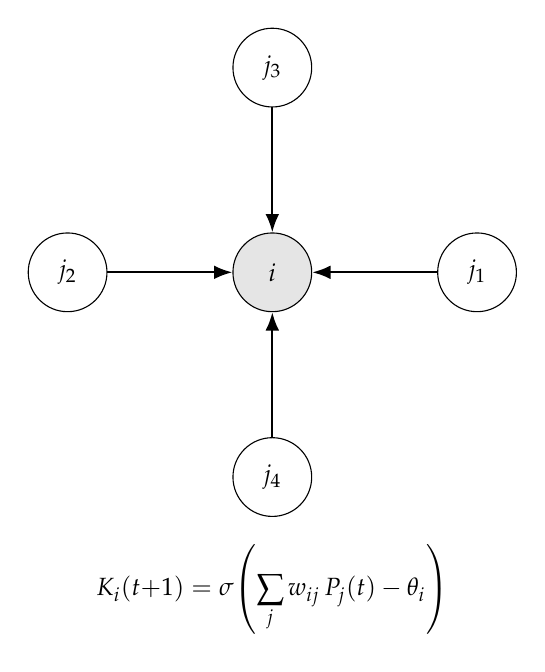
\begin{tikzpicture}[
    scale=1.3,
    node/.style={circle, draw, minimum size=1cm, inner sep=0pt, font=\small},
    arrow/.style={-{Latex}, thick}
]
\node[node, fill=gray!20] (c) at (0,0) {$i$};
\node[node] (n1) at ( 2.0, 0) {$j_1$};
\node[node] (n2) at (-2.0, 0) {$j_2$};
\node[node] (n3) at (0,  2.0) {$j_3$};
\node[node] (n4) at (0, -2.0) {$j_4$};
\draw[arrow] (n1) -- (c);
\draw[arrow] (n2) -- (c);
\draw[arrow] (n3) -- (c);
\draw[arrow] (n4) -- (c);
\node[draw=none, font=\small] at (0,-3.1) {$K_i(t{+}1) = \sigma\!\left(\displaystyle\sum_j w_{ij}\, P_j(t) - \theta_i\right)$};
\end{tikzpicture}
\caption{Local update rule of a knot lattice node $i$ driven by pressure inputs from neighboring nodes $j_1,\ldots,j_4$. No global coordination occurs; routing decisions emerge from local pressure conditions alone.}
\end{figure}

The most novel component of the reactor is the knot lattice, which operates as a distributed computational system by translating local pressure conditions into routing decisions without any centralized processing. In a recurrent formulation, each node $i$ evolves according to:
\[
K_i(t+1) = \sigma \!\left( \sum_j w_{ij}\, P_j(t) - \theta_i \right)
\]
where $P_j(t)$ is the pressure at neighboring node $j$, $w_{ij}$ are coupling coefficients encoding the hydraulic connectivity of the network, and $\sigma$ is a threshold function. Unlike digital systems, computation here is continuous in time, spatially distributed across the physical domain, and directly coupled to energy flow. The system effectively solves a routing and optimization problem:
\[
\min_{\{K_i\}} \Bigl( \mathcal{L}_{\text{flow}} + \lambda\, \mathcal{L}_{\text{energy}} + \beta\, \mathcal{L}_{\text{wear}} \Bigr)
\]
without explicit symbolic processing. The three loss terms penalize respectively suboptimal flow paths, excess energy expenditure, and mechanical wear on the lattice nodes.

\section{AI-Augmented Control Layer}

An external convolutional neural network processes Raman spectral data from the biomass, mapping raw spectra $S_{\text{raw}}(\lambda)$ to a classification of material state. This classification selects optimal press parameters and material handling strategies, augmenting the purely physical computation of the knot lattice with statistical inference over composition. The combined system is therefore hybrid in character: physical computation through the pressure-driven lattice handles fast, spatially local routing decisions, while the neural inference layer handles slower, globally informed adaptation of cycle parameters.

\section{Biological Integration}

Engineered yeast strains are introduced into the biomass column to perform catalytic conversion during and between press cycles. The primary catalytic functions are glucoamylase production for polysaccharide hydrolysis, lipase activity for triglyceride breakdown, and the synthesis of polyhydroxyalkanoates (PHA) from available carbon substrates. These biochemical transformations are embedded directly into the mechanical cycle rather than being confined to a separate bioreactor stage, so that the compression and thermal gradients of the press phase serve simultaneously as the mechanical and energetic drivers of the catalytic reactions.

\section{Variational Formulation of the Knot Lattice}

The thermofluidic knot lattice can be formalized not merely as a discrete switching system, but as the minimizer of an underlying functional defined over pressure fields and routing states. This variational formulation elevates the computational layer from a heuristic neural analogy to a field-theoretic object with well-defined dynamical properties.

\subsection{State Representation}

Let the system be defined over a spatial domain $\Omega \subset \mathbb{R}^3$. At each point $x \in \Omega$, we define the joint state:
\[
X(x,t) = \bigl(P(x,t),\;\mathbf{u}(x,t),\;K(x,t)\bigr)
\]
where $P(x,t)$ is the pressure field, $\mathbf{u}(x,t)$ is the fluid velocity, and $K(x,t) \in [-1,1]$ is a continuous relaxation of the knot state. The discrete switching behavior emerges as a limiting case of this continuous representation under strong potential barriers, as made precise below.

\subsection{Energy Functional}

We define a global functional $\mathcal{J}$ governing the system:
\[
\mathcal{J}[P,\mathbf{u},K] =
\int_{\Omega}
\Bigl(
\alpha \|\nabla P\|^2
+ \beta \|\mathbf{u}\|^2
+ \gamma V(K)
+ \delta K\, P
\Bigr) dV
\]

\begin{figure}[h]
\centering
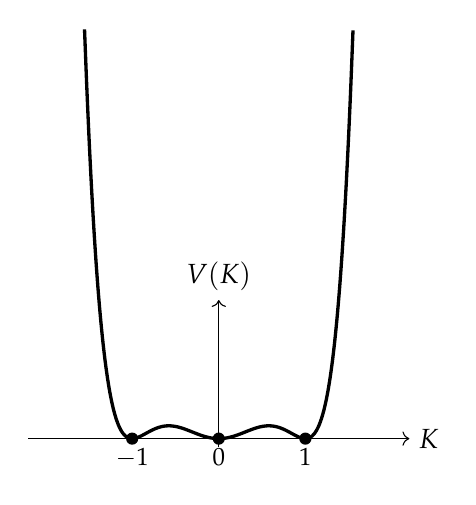
\begin{tikzpicture}[scale=1.1]
\draw[->] (-2.2,0) -- (2.2,0) node[right] {$K$};
\draw[->] (0,-0.1) -- (0,1.6) node[above] {$V(K)$};
\draw[domain=-1.55:1.55, smooth, very thick, samples=120]
    plot (\x, {(\x+1)*(\x+1)*(\x)*(\x)*(\x-1)*(\x-1)});
\node[below, font=\small] at (-1, 0) {$-1$};
\node[below, font=\small] at ( 0, 0) {$0$};
\node[below, font=\small] at ( 1, 0) {$1$};
\foreach \x in {-1, 0, 1}
    \fill (\x, 0) circle (2pt);
\end{tikzpicture}
\caption{Triple-well potential $V(K) = (K+1)^2 K^2 (K-1)^2$ governing knot state stability. The three minima at $K = -1, 0, 1$ correspond to reverse routing, passive, and forward routing configurations respectively. The discrete ternary logic of the knot lattice emerges from these wells in the limit $\gamma \to \infty$.}
\end{figure}

The term $\|\nabla P\|^2$ penalizes steep pressure gradients and thereby regularizes the spatial structure of the pressure field. The term $\|\mathbf{u}\|^2$ captures kinetic energy cost, disfavoring flows whose magnitude is not justified by the routing task. The potential $V(K)$ is a double-well (triple-well) function enforcing the ternary discrete structure; a natural choice is:
\[
V(K) = (K+1)^2\, K^2\, (K-1)^2
\]
which creates stable minima at $K = -1,\, 0,\, 1$ and barriers between them. The coupling term $\delta K P$ directly links routing decisions to the local pressure field, so that regions of high pressure bias nodes toward their active states.

\subsection{Euler--Lagrange Dynamics}

The system evolves toward minimizing $\mathcal{J}$ by gradient descent in the function space of $(P, \mathbf{u}, K)$. The resulting equations of motion are:
\[
\frac{\partial P}{\partial t} = -\frac{\delta \mathcal{J}}{\delta P} = \alpha\, \Delta P - \delta K
\]
\[
\frac{\partial K}{\partial t} = -\frac{\delta \mathcal{J}}{\delta K} = -\gamma\, V'(K) - \delta P
\]
\[
\frac{\partial \mathbf{u}}{\partial t} = -\frac{\delta \mathcal{J}}{\delta \mathbf{u}} = -2\beta\, \mathbf{u}
\]
These equations define a coupled relaxation system in which pressure smooths spatially toward configurations that balance diffusion against coupling to the knot state, knot states align with local pressure conditions while resisting displacement from the potential wells, and flow dissipates unless driven by external forcing.

\subsection{Discrete Switching as a Limit}

The original ternary logic $K \in \{-1, 0, 1\}$ emerges in the strong-barrier limit $\gamma \to \infty$, which forces $K$ into the minima of $V(K)$ and makes the potential barriers effectively infinite. In this limit the continuous relaxation collapses to the discrete switching rule of Section~4.1, so the discrete fluidic logic is not a fundamental description but a coarse-grained projection of the continuous variational dynamics onto its attractor set.

\subsection{Interpretation as Physical Inference}

The minimization of $\mathcal{J}$ can be interpreted as a form of distributed inference over the domain $\Omega$:
\[
\min_{K} \;\mathbb{E}_{x \in \Omega}
\bigl[
\text{energy cost} + \text{routing mismatch}
\bigr]
\]
In this view, $P(x,t)$ acts as a data field encoding the current energetic state of the system, $K(x,t)$ encodes local routing decisions, and the system collectively infers an optimal routing configuration by evolving the coupled field equations. External inputs such as steam injection and cooling rates enter as forcing terms modifying the pressure equation:
\[
\frac{\partial P}{\partial t} = \alpha\, \Delta P - \delta K + f_{\text{ext}}(x,t)
\]
Control is therefore exerted not by direct routing commands but by shaping the energy landscape, which alters the equilibrium toward which the self-organizing field relaxes.

\section{Correspondence with Field-Theoretic Systems}

The variational structure established above places the Caldera Reactor within the class of dissipative field systems with internal state coupling:
\[
\frac{dX}{dt} = -\nabla_X \mathcal{J} + F_{\text{ext}}
\]
Three properties of this class are directly realized in the reactor. Computation arises from gradient descent in a physical functional rather than from any symbolically specified algorithm. Routing decisions correspond to local minima selection in the joint configuration space of $(P, K)$. Global coordination emerges without centralized control because the functional $\mathcal{J}$ is defined over the entire domain and its gradient descent propagates influence across all connected regions.

\subsection{Relation to Entropy and Accessibility}

The knot state $K$ can be interpreted as a constraint field regulating the set of accessible flow configurations. Regions where $K$ is unstable—transitional zones between the potential wells—correspond to high configurational variability, where a small perturbation in pressure can redirect flow across several routing options. Stable regions, by contrast, enforce constrained dynamics: the flow is locked to a particular path and insensitive to small fluctuations. This spatial variation in configurational accessibility provides a natural bridge to entropy-like measures, which we make precise in the RSVP reinterpretation below.

\section{RSVP Reinterpretation of the Caldera Reactor}

The Caldera Reactor can be recast within the Relativistic Scalar--Vector Plenum (RSVP) framework by identifying its physical fields with the canonical RSVP state triple:
\[
X(x,t) = \bigl(\Phi(x,t),\;\mathbf{v}(x,t),\;S(x,t)\bigr)
\]

\begin{figure}[h]
\centering
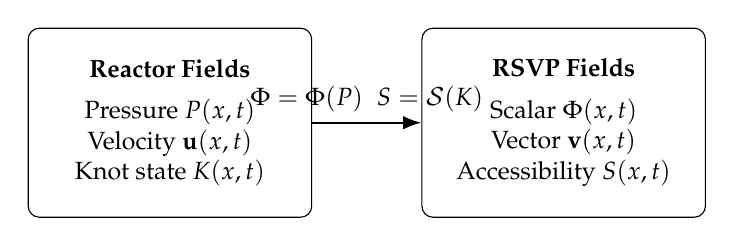
\begin{tikzpicture}[
    node distance=5cm,
    box/.style={draw, rectangle, rounded corners, minimum width=3.6cm, minimum height=2.4cm, align=center, font=\small},
    arrow/.style={-{Latex}, thick}
]
\node[box] (reactor) {
\textbf{Reactor Fields}\\[4pt]
Pressure $P(x,t)$\\
Velocity $\mathbf{u}(x,t)$\\
Knot state $K(x,t)$
};
\node[box, right of=reactor] (rsvp) {
\textbf{RSVP Fields}\\[4pt]
Scalar $\Phi(x,t)$\\
Vector $\mathbf{v}(x,t)$\\
Accessibility $S(x,t)$
};
\draw[arrow] (reactor) -- node[above, font=\small]{$\Phi = \Phi(P)$\;\;$S = \mathcal{S}(K)$} (rsvp);
\end{tikzpicture}
\caption{Structural mapping between Caldera Reactor fields and RSVP state variables. The pressure field maps to the scalar potential via a monotonic proxy; the knot state maps to the accessibility field via a stability functional.}
\end{figure}

To make the correspondence precise, we interpret the pressure field $P(x,t)$ not as the scalar potential itself, but as a physically realized proxy for a generalized potential $\Phi(x,t)$, related by a monotonic mapping $\Phi = \Phi(P)$ that preserves ordering and gradient structure. This avoids conflating pressure with a scalar potential in the general field-theoretic sense while retaining the full structural equivalence. The reinterpretation therefore expresses a structural equivalence arising directly from the governing dynamics.

\subsection{Field Correspondence}

The mapping between reactor fields and RSVP fields is as follows. The pressure field $P(x,t)$ corresponds to the scalar potential $\Phi(x,t)$: both act as the primary driving field that propagates influence through the medium and determines the energetic bias on local state variables. The fluid velocity $\mathbf{u}(x,t)$ corresponds to the transport field $\mathbf{v}(x,t)$: both encode the directed propagation of energy and material through the domain. The knot state $K(x,t)$ is mapped to the accessibility field $S(x,t)$ via a monotonic functional $\mathcal{S}[K]$ measuring the stability or degeneracy of knot configurations. Concretely, stable discrete states $K \in \{-1, 0, 1\}$ correspond to low-accessibility regions ($S \downarrow$), while transitional regions where $K$ fluctuates correspond to high-accessibility regions ($S \uparrow$). The knot lattice thus induces a spatially varying accessibility field whose geometry is determined by the pressure distribution.

\subsection{Dynamical Equivalence}

The variational dynamics of Section~9 can be rewritten in RSVP form as:
\[
\frac{\partial \Phi}{\partial t} = D_\Phi\, \Delta\Phi + F_\Phi(S) + f_{\text{ext}}
\]
\[
\frac{\partial S}{\partial t} = -\nabla_\Phi\, \mathcal{C}(\Phi, S)
\]
\[
\frac{\partial \mathbf{v}}{\partial t} = -\lambda\, \mathbf{v} + F_{\text{drive}}(\Phi)
\]
where $F_\Phi(S)$ captures constraint-mediated feedback (corresponding to the $-\delta K$ term in the pressure equation), $\mathcal{C}(\Phi, S)$ is an effective constraint potential whose gradient drives accessibility toward configurations consistent with the local scalar field, and $F_{\text{drive}}(\Phi)$ encodes pressure-driven flow coupling. These three equations match the general RSVP form for a coupled system of scalar, vector, and accessibility fields.

\subsection{Constraint Closure and Knot Stability}

In RSVP, stable structures arise from constraint closure: configurations in which admissible trajectories are self-consistent across scales, so that the field equations reinforce rather than contradict each other. In the Caldera system, closure occurs when:
\[
\frac{\partial K}{\partial t} \approx 0
\quad\text{and}\quad
\frac{\partial P}{\partial t} \approx 0
\]
which, substituting into the Euler--Lagrange equations, yields the condition:
\[
\gamma\, V'(K) + \delta P \approx 0
\]
This condition defines a local equilibrium between pressure gradients and routing constraints. Knot stability therefore corresponds exactly to constraint closure in the RSVP sense, and pressure alignment across the domain corresponds to admissible trajectory flow through the space of possible routing configurations.

\subsection{Entropy as Accessibility of Flow Configurations}

Unlike thermodynamic entropy in equilibrium systems, the effective entropy field $S(x,t)$ here measures the logarithmic volume of admissible routing configurations in the neighborhood of each point:
\[
S(x,t) \;\sim\; \log \bigl( \#\text{ admissible flow paths near } x \bigr)
\]
Regions of high $S$ are characterized by unstable knot states, high configurational flexibility, and increased sensitivity to perturbations; small changes in pressure can redirect flow through several alternative paths. Regions of low $S$ are characterized by locked routing configurations, efficient energy transfer along constrained paths, and reduced dynamical freedom. This interpretation aligns directly with RSVP's definition of entropy as the accessibility measure over future trajectory branches, extended here from an abstract field-theoretic setting to a concrete physical substrate.

\subsection{Energy Flow as Entropy Descent}

The reactor cycle can be interpreted as a structured sequence of entropy descent phases. Steam injection increases $\Phi$ and expands the set of accessible configurations ($S \uparrow$). Condensation and routing collapse reduce accessibility as the system selects among the available paths ($S \downarrow$). Compression enforces constraint closure by eliminating remaining configurational degeneracy and extracting usable work. Energy extraction thus corresponds to the transition:
\[
S_{\text{high}} \;\rightarrow\; S_{\text{low}}
\]
driven by structured constraint imposition rather than by random thermal fluctuation. The directedness of this entropy descent—the fact that it follows the gradient of $\mathcal{J}$ rather than diffusing randomly—is precisely what makes the reactor an engine rather than a thermal bath.

\subsection{Emergent Computation as RSVP Dynamics}

Within this framework, computation is not an added feature of the reactor but an intrinsic property of the field dynamics. The scalar field $\Phi$ encodes the driving signal; the vector field $\mathbf{v}$ propagates influence across the domain; and the accessibility field $S$ regulates which transitions are admissible at each point. The system computes by evolving toward configurations where $(\Phi, \mathbf{v}, S)$ satisfy mutual consistency constraints—that is, toward states of constraint closure. This is equivalent to solving a constrained optimization problem over trajectory space, but the optimization is performed by the physical dynamics themselves rather than by any external algorithm.

\subsection{Implications for Reactor Design}

The RSVP reinterpretation suggests several new design principles that are not visible from the engineering description alone. First, useful work is maximized by engineering large, controlled gradients in $\Phi$ to drive flow, rather than by simply increasing total pressure. Second, the geometry of the knot lattice should be designed to shape the $S$ landscape—the spatial distribution of accessibility—so that entropy descent follows a path that maximizes energy recovery per cycle. Third, coupling coefficients between $\Phi$ and $S$ should be tuned to enforce rapid constraint closure without inducing oscillatory instability, a condition that can be characterized precisely in terms of the spectral properties of the linearized system. These principles reframe the reactor as a programmable field system whose performance is determined by landscape geometry rather than by component specifications.

\section{Extended State Representation and Global Evolution}

Incorporating the biochemical layer, the full reactor state can be represented as:
\[
X(t) = (P,\, V,\, K,\, B)
\]
where $P$ is the pressure field, $V$ encodes the volume and geometry of the compression chamber, $K$ is the computational state of the knot lattice, and $B$ is the biochemical composition of the biomass column. The global evolution operator is:
\[
\frac{dX}{dt} = \mathcal{F}(X, u, \theta)
\]
where $u$ denotes external inputs (steam injection rate, cooling schedule, spectral control signals) and $\theta$ denotes the fixed parameters of the system (geometric constants, material properties, biological strain characteristics). This places the Caldera Reactor within the class of adaptive thermodynamic machines with embedded computation: systems in which the control mechanism is not separate from the physical process but constitutive of it.

\section{Numerical Discretization and Simulation Correspondence}

To establish the operational equivalence between the reactor dynamics and the RSVP framework, we construct a discrete approximation of the coupled field system. This serves both as a simulation model and as a constructive realization of the variational dynamics, converting the structural claim of equivalence into an explicit algorithmic correspondence.

\subsection{Spatial Discretization}

Let the domain $\Omega$ be discretized into a regular lattice of cells indexed by $i$, each carrying the local state $X_i(t) = (P_i(t), \mathbf{u}_i(t), K_i(t))$. Spatial derivatives are approximated using nearest-neighbor stencils; in particular, the Laplacian of the pressure field is given by:
\[
\Delta P_i \;\approx\; \sum_{j \in \mathcal{N}(i)} (P_j - P_i)
\]
where $\mathcal{N}(i)$ denotes the set of cells neighboring cell $i$. This stencil preserves the local character of the physical interactions: each cell's update depends only on its immediate neighborhood, so the decentralized structure of the continuous system is inherited by the discrete approximation.

\subsection{Discrete Evolution Equations}

The continuous Euler--Lagrange system yields the following explicit discrete-time update rules under timestep $\Delta t$:
\[
P_i^{t+1} = P_i^t + \Delta t \left( \alpha \sum_{j \in \mathcal{N}(i)} (P_j^t - P_i^t) - \delta K_i^t + f_i^t \right)
\]
\[
K_i^{t+1} = K_i^t + \Delta t \left( -\gamma V'(K_i^t) - \delta P_i^t \right)
\]
\[
\mathbf{u}_i^{t+1} = (1 - 2\beta \Delta t)\, \mathbf{u}_i^t + \Delta t\, F_{\text{drive}}(P_i^t)
\]
Each cell evolves based only on its current state and the states of its neighbors. The external forcing term $f_i^t$ encodes steam injection or cooling inputs at cell $i$ and time $t$, entering the pressure equation as an additive source.

\subsection{Recovery of Discrete Logic}

In the strong-barrier limit $\gamma \gg 1$, the knot potential $V(K)$ becomes effectively infinite outside the minima, and the knot state rapidly converges to $K_i \in \{-1, 0, 1\}$. In this regime the update rule for $K$ reduces to a thresholded pressure response:
\[
K_i^{t+1} \approx \mathrm{sign}(P_i^t - \theta_i)
\]
recovering the original fluidic switching logic of Section~4.1. The discrete control behavior observed in the physical reactor is thus reproduced as a limiting case of the continuous simulation, which confirms that the variational formulation is not an independent model but a generalization of the engineering description.

\subsection{Correspondence with RSVP Simulation}

Under the identification $\Phi_i \equiv P_i$, $\mathbf{v}_i \equiv \mathbf{u}_i$, and $S_i \equiv \mathcal{S}(K_i)$, the discrete update rules take the canonical RSVP form:
\[
\Phi_i^{t+1} = \Phi_i^t + \Delta t \left( D_\Phi\, \Delta \Phi_i^t + F_\Phi(S_i^t) + f_i^t \right)
\]
\[
S_i^{t+1} = S_i^t + \Delta t\, G(\Phi_i^t, S_i^t)
\]
\[
\mathbf{v}_i^{t+1} = (1 - \lambda \Delta t)\, \mathbf{v}_i^t + \Delta t\, F_{\text{drive}}(\Phi_i^t)
\]
This structure is identical to that of the discrete RSVP field simulator previously developed within the framework. The equivalence is therefore not merely formal but algorithmic: the same update rules that simulate RSVP dynamics simulate the Caldera Reactor under appropriate parameter choices, and the same class of update rules, under appropriate parameterization, serves both purposes.

\subsection{Stability and Convergence}

The stability of the discrete system is governed by standard conditions on $\Delta t$ and the coupling coefficients. Diffusion stability in $d$ spatial dimensions requires:
\[
\Delta t < \frac{1}{2d\alpha}
\]
Stability of the knot dynamics requires in addition that the effective stiffness $\gamma$ not induce oscillatory overshoot in the $K$ update, which is satisfied when $\gamma \Delta t \max_K |V''(K)| < 2$. Under these conditions the system converges toward fixed points of the coupled update, corresponding to constraint-closed configurations in which $\partial K / \partial t \approx 0$ and $\partial P / \partial t \approx 0$ simultaneously.

\subsection{The Physical Process as Continuous Computation}

This discretization demonstrates that the reactor dynamics are not only formally equivalent to RSVP but are algorithmically realizable as a local update rule over a lattice. The physical reactor can therefore be interpreted as executing, in continuous time, the same field-theoretic computation that a discrete RSVP simulator performs in iterative steps. The distinction between physical process and simulation becomes structurally minimal: the reactor realizes, in continuous time, the same local update dynamics that a discrete RSVP simulator approximates iteratively, running on conventional hardware under identical governing equations. This constructive correspondence closes the gap between the paper's structural claims and their operational content.


\section{Conclusion}

The Caldera Reactor represents a synthesis of thermodynamics, computation, and biological processing whose deepest interest lies not in any single component but in the way these levels of description interact. The engineering dynamics of the press cycle, the variational field theory of the knot lattice, and the RSVP reinterpretation of the coupled fields are not three separate accounts of the same system but three levels of resolution of a single coherent object.

The variational formulation shows that the discrete switching logic of the knot lattice is not an independently designed control system but an emergent consequence of gradient descent in a physically grounded energy functional. The RSVP reinterpretation shows that this gradient descent is structurally identical to the field dynamics of constraint-mediated inference, establishing the reactor as a concrete physical realization of RSVP dynamics at the mesoscale. The key innovation—the collapse of the boundary between control and mechanism—thus has a precise theoretical expression: computation arises because the system's energy functional couples the state of the medium to the admissibility of its own trajectories.

This suggests a broader design paradigm in which industrial systems are constructed as self-optimizing dynamical fields rather than centrally controlled machines, and in which the concept of computation is not imposed on a physical system from outside but recognized as an intrinsic feature of any field system that evolves toward constrained accessibility minima. The reactor thus provides not only a promising engineering platform but a validation domain for the theoretical claims of the RSVP framework, one in which the abstract notions of constraint closure, accessibility descent, and emergent inference can be subjected to direct experimental test. In this formulation, energy storage, transport, and computation are not separable subsystems but different aspects of a single field evolution, distinguished only by the observables through which they are measured. In this sense, conventional thermal storage systems correspond to the scalar limit of a more general field-theoretic class, of which the Caldera Reactor provides a concrete realization---and the numerical discretization established above ensures that this realization is not merely interpretive but computationally exact.


\appendix

\section{Algorithmic Implementation of the Discrete Field Dynamics}

This appendix provides a constructive implementation of the discrete field dynamics introduced in Section~12. The goal is to make explicit the local update rules governing the evolution of the pressure field $P$, velocity field $\mathbf{u}$, and knot state $K$, and to demonstrate how these rules can be realized as a lattice-based simulation requiring no centralized coordination.

\subsection{Discrete State Variables}

We consider a regular lattice of cells indexed by $i \in \Lambda$, each storing the local state $X_i^t = (P_i^t, \mathbf{u}_i^t, K_i^t)$, where $P_i^t \in \mathbb{R}$ is the pressure, $\mathbf{u}_i^t \in \mathbb{R}^3$ is the velocity vector, and $K_i^t \in [-1,1]$ is the relaxed knot state. These three variables correspond under the RSVP mapping to $\Phi_i$, $\mathbf{v}_i$, and $\mathcal{S}(K_i)$ respectively.

\subsection{Neighborhood Structure and Discrete Laplacian}

Each cell interacts with a finite set of neighbors $\mathcal{N}(i)$. For a cubic lattice in three dimensions, this is typically the six-face neighborhood or the twenty-six-cell neighborhood including diagonals. The discrete Laplacian of the pressure field is:
\[
\Delta P_i^t = \sum_{j \in \mathcal{N}(i)} (P_j^t - P_i^t)
\]
This stencil is local by construction: each cell's contribution to its own update is determined entirely by the difference between its pressure and those of its immediate neighbors.

\subsection{Update Equations and Potential Derivative}

At each timestep $t \to t+1$, the three fields are updated by:
\[
P_i^{t+1} = P_i^t + \Delta t \left( \alpha \sum_{j \in \mathcal{N}(i)} (P_j^t - P_i^t) - \delta K_i^t + f_i^t \right)
\]
\[
K_i^{t+1} = K_i^t + \Delta t \left( -\gamma V'(K_i^t) - \delta P_i^t \right)
\]
\[
\mathbf{u}_i^{t+1} = (1 - 2\beta \Delta t)\, \mathbf{u}_i^t + \Delta t\, F_{\text{drive}}(P_i^t)
\]
The triple-well potential and its derivative, required for the knot update, are:
\[
V(K) = (K+1)^2 K^2 (K-1)^2
\qquad
V'(K) = 6K^5 - 8K^3 + 2K
\]

\subsection{Boundary Conditions}

Three boundary condition types are appropriate for different simulation regimes. Dirichlet conditions fix the pressure at boundary cells, modeling inlet or outlet regions with prescribed values. Neumann conditions impose zero normal gradient at closed walls, appropriate where no fluid crosses the boundary. Periodic conditions identify opposite faces of the domain, suitable for idealized or toroidal geometries. External forcing $f_i^t$ is applied at selected boundary or interior nodes to model steam injection (positive forcing) or cooling (negative forcing).

\subsection{Simulation Algorithm}

The full update procedure is as follows. Given initial fields $P_i^0$, $K_i^0$, $\mathbf{u}_i^0$ and parameters $\alpha, \beta, \gamma, \delta, \Delta t$, at each timestep one computes the discrete Laplacian for every cell, then updates $P$, $K$, and $\mathbf{u}$ in parallel using the equations above, then applies boundary conditions and advances $t$:

\begin{verbatim}
Initialize P_i, K_i, u_i for all cells i
Set parameters alpha, beta, gamma, delta, dt

for each timestep t:
    for each cell i:
        lapP = sum_{j in N(i)} (P_j - P_i)

        P_new[i] = P_i + dt*(alpha*lapP - delta*K_i + f_i)
        K_new[i] = K_i + dt*(-gamma*V_prime(K_i) - delta*P_i)
        u_new[i] = (1 - 2*beta*dt)*u_i + dt*F_drive(P_i)

    apply boundary conditions

    P_i = P_new[i];  K_i = K_new[i];  u_i = u_new[i]
\end{verbatim}

The update is fully local: each cell reads only its own state and those of its neighbors, writing to a temporary buffer before the global overwrite. No global communication or centralized coordination occurs at any stage.

\subsection{Optional Discrete Projection}

To recover the original ternary knot logic from the continuous relaxation, one may apply a projection step after each $K$ update:
\[
K_i^{t+1} \;\leftarrow\;
\begin{cases}
\phantom{-}1 & \text{if } K_i^{t+1} > \theta_+ \\
-1 & \text{if } K_i^{t+1} < \theta_- \\
\phantom{-}0 & \text{otherwise}
\end{cases}
\]
where $\theta_+$ and $\theta_-$ are symmetrically placed thresholds close to the potential minima. In the limit $\gamma \to \infty$ this projection becomes redundant, as the continuous dynamics force $K$ into the minima automatically.

\subsection{Stability Parameters and Constraints}

Numerical stability requires two conditions to hold simultaneously. The diffusion stability condition for a $d$-dimensional lattice is $\Delta t < 1/(2d\alpha)$, preventing oscillatory growth in the pressure update. The knot stability condition $\gamma \Delta t \max_K |V''(K)| < 2$ prevents overshoot in the potential gradient term; since $\max_K |V''(K)|$ is bounded and computable from the analytic form of $V$, this condition can be enforced at initialization. Representative parameter choices for a two-dimensional test simulation are $\alpha = 0.1$, $\beta = 0.05$, $\gamma = 2.0$, $\delta = 0.3$, and $\Delta t = 0.05$.

\subsection{Correspondence with RSVP Simulation}

Under the mapping $\Phi_i \equiv P_i$, $\mathbf{v}_i \equiv \mathbf{u}_i$, $S_i \equiv \mathcal{S}(K_i)$, the algorithm above is structurally identical to the discrete RSVP field simulator previously developed within the framework. The pressure propagation step corresponds to scalar field diffusion with constraint feedback; the knot update corresponds to accessibility field relaxation driven by the scalar potential; and the velocity update corresponds to transport field dissipation with pressure-driven forcing. The same class of update rules, under appropriate parameterization, therefore simulates both systems without modification. This algorithmic identity is the constructive content of the Caldera--RSVP correspondence: not merely that the two systems share a mathematical form, but that a single implementation realizes both.



\begin{thebibliography}{99}

\bibitem{caldera0}
Flyxion.
\newblock Caldera Reactor: Original Design Proposal (Version 0).
\newblock Unpublished technical document, 2024.

\bibitem{rsvp}
Flyxion.
\newblock {RSVP--Polyxan: A Unified Field Theory of Semantic Hyperstructures}.
\newblock Unpublished monograph, 2024.

\bibitem{yarncrawler}
Flyxion.
\newblock Yarncrawler: World-State Reconstruction as Constraint Closure.
\newblock Unpublished monograph, 2024.

\bibitem{tidal}
A.~S. Bahaj.
\newblock Generating electricity from the oceans.
\newblock \emph{Renewable and Sustainable Energy Reviews}, 15(7):3399--3416, 2011.

\bibitem{tidal2}
I.~G. Bryden and S.~J. Couch.
\newblock Marine energy extraction: tidal resource analysis.
\newblock \emph{Renewable Energy}, 31(2):133--139, 2006.

\bibitem{pyrolysis}
M.~Lewan.
\newblock Experiments on the role of water in petroleum formation.
\newblock \emph{Geochimica et Cosmochimica Acta}, 61(17):3691--3723, 1997.

\bibitem{hydrous}
D.~W. Houseknecht.
\newblock Assessing hydrocarbon generation via hydrous pyrolysis.
\newblock \emph{AAPG Bulletin}, 87(6):909--924, 2003.

\bibitem{kelp}
T.~Chopin et al.
\newblock Seaweed aquaculture for sustainable food systems.
\newblock \emph{Nature Sustainability}, 5:973--983, 2022.

\bibitem{kelp2}
C.~M. Duarte et al.
\newblock Can seaweed farming play a role in climate change mitigation?
\newblock \emph{Nature Climate Change}, 7:737--742, 2017.

\bibitem{tes_review}
S.~Chavan, R.~Rudrapati, and S.~Manickam.
\newblock Advances in thermal energy storage and applications.
\newblock \emph{Alexandria Engineering Journal}, 61(7):5455--5463, 2022.

\bibitem{sand_battery}
Siswanto, Rusdianasari, and Indrayani.
\newblock Performance improvement of sand-based batteries using sea sand and metal waste as an alternative energy storage system.
\newblock \emph{International Journal of Research in Vocational Studies}, 5(2):1--7, 2025.

\bibitem{tes_conductivity}
J.~Wang et al.
\newblock Predictive models for thermal conductivity of sands.
\newblock \emph{Energies}, 13(5):1083, 2020.

\bibitem{hybrid_storage}
A.~M. Adeyinka et al.
\newblock Hybrid energy storage systems for renewable integration.
\newblock \emph{Sustainable Energy Research}, 11(1), 2024.

\end{thebibliography}

\end{document}
